% PhaseWall in two pages: schematics and examples, short statements only.
% Figures: python docs/tldr/make_crops.py and python docs/tldr/make_figures.py (from the repository).
% Build: pdflatex TLDR.tex; cp TLDR.pdf ../TLDR.pdf
\documentclass[10pt]{article}
\usepackage[a4paper,landscape,margin=6mm]{geometry}
\usepackage{amsmath,amssymb}
\usepackage[scaled]{helvet}
\renewcommand\familydefault{\sfdefault}
\usepackage[T1]{fontenc}
\usepackage{graphicx}
\usepackage{xcolor}
\usepackage{tikz}
\usetikzlibrary{arrows.meta,positioning,calc}
% Shared colours and styles of the schematics (input once in the preamble).
% The phase colours are those of phasewall.report, so schematics and data figures agree.
\definecolor{cP0}{HTML}{2A78D6}    % phase 0 (stripes in the demo)
\definecolor{cP1}{HTML}{EB6834}    % phase 1 (hexagons)
\definecolor{cP2}{HTML}{1BAF7A}    % phase 2 (uniform)
\definecolor{cInk}{HTML}{0B0B0B}
\definecolor{cInk2}{HTML}{52514E}
\definecolor{cGrid}{HTML}{C9C8C3}
\definecolor{cNeg}{HTML}{184F95}   % negative values (field maps)
\definecolor{cPos}{HTML}{B23A39}   % positive values
\definecolor{cAcc}{HTML}{D55E00}   % accent: thresholds, the wall

\tikzset{
  fig/.style={font=\small, >={Stealth}},
  lab/.style={font=\footnotesize\bfseries, align=center},
  note/.style={font=\footnotesize, align=center},
  small/.style={font=\scriptsize, align=center},
  blk/.style={draw, rounded corners, align=center, font=\footnotesize, inner sep=4pt, fill=black!3},
  dot/.style={circle, fill=#1, inner sep=0pt, minimum size=4pt},
  wall/.style={cAcc, line width=1.4pt},
}

\definecolor{cOK}{HTML}{1B8A5A}
\definecolor{cBad}{HTML}{B23A39}
\pagestyle{empty}
\tikzset{
  box/.style={draw=cInk2, rounded corners=3pt, line width=0.6pt, fill=white},
  head/.style={font=\bfseries\small, anchor=north west},
  say/.style={font=\footnotesize, anchor=north west, align=left},
  num/.style={circle, fill=cInk, text=white, font=\bfseries\scriptsize, inner sep=1.5pt},
  tile/.style={draw=cInk2, line width=0.4pt, minimum size=0.55cm, inner sep=0pt},
  big/.style={->, line width=2pt, cInk2},
}
% a square of stripes: centre, half side, rotation, spacing, colour strength
\newcommand{\stripes}[5]{%
  \begin{scope}[shift={#1}, rotate=#3]
    \fill[white] (-#2,-#2) rectangle (#2,#2);
    \begin{scope} \clip (-#2,-#2) rectangle (#2,#2);
      \pgfmathsetmacro{\stripestep}{-1.6+#4}
      \foreach \s in {-1.6,\stripestep,...,1.6} \draw[cPos!#5, line width=1.3pt] (\s,-#2-0.2) -- (\s,#2+0.2);
    \end{scope}
    \draw[cInk2, line width=0.5pt] (-#2,-#2) rectangle (#2,#2);
  \end{scope}}
\begin{document}
%====================================================================== page 1
\noindent\resizebox{\linewidth}{!}{%
\begin{tikzpicture}[x=1cm,y=1cm,>={Stealth}]
\node[anchor=north west, font=\bfseries\Large] at (0,0) {PhaseWall: find the phases of a simulated system, without labels};

% ---------------- the problem in one picture
\node[anchor=north west, font=\bfseries\normalsize] at (0,-0.85) {What you have: many runs on a parameter grid};
\node[anchor=north west, inner sep=0] at (0,-1.4) {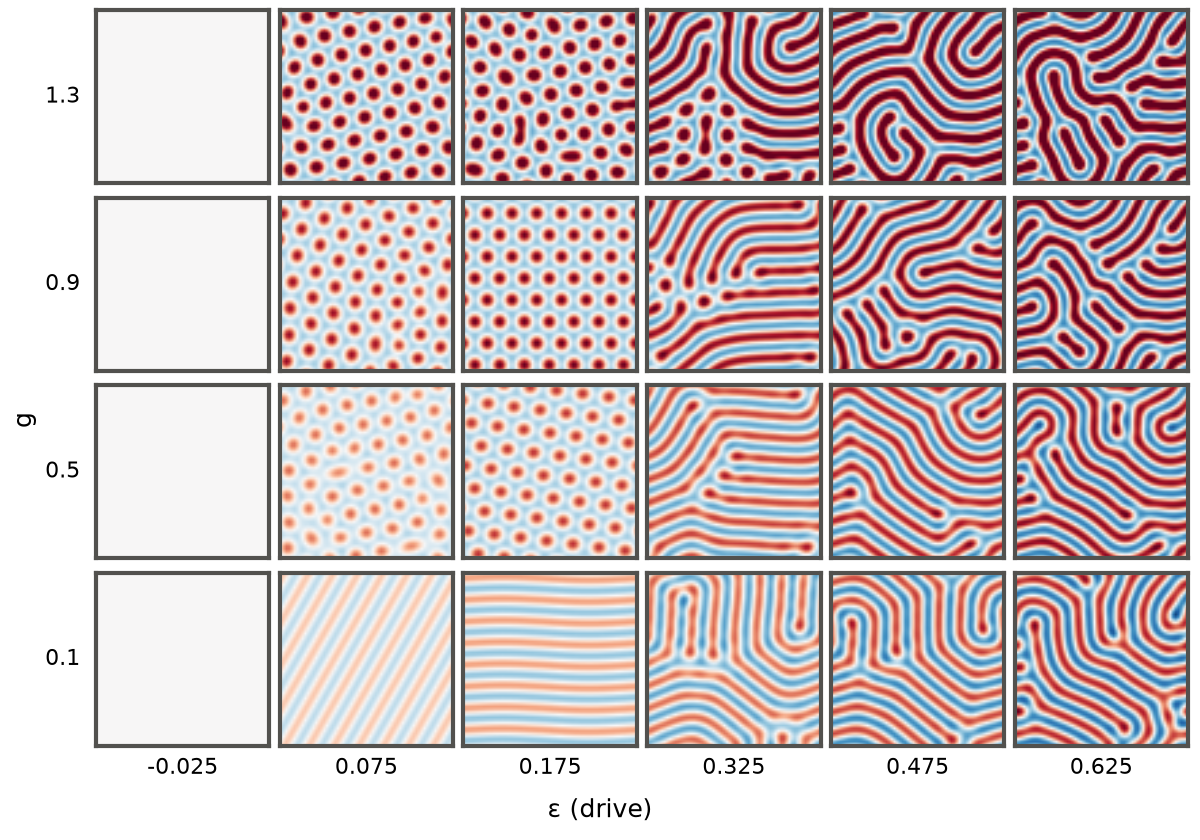
\includegraphics[height=6.6cm]{fig_sh_grid.png}};
\draw[big] (9.75,-4.6) -- (11.65,-4.6);
\node[font=\bfseries\small, align=center] at (10.7,-4.0) {PhaseWall};
\node[font=\footnotesize, align=center] at (10.7,-5.2) {no labels\\no number\\of phases};
\node[anchor=north west, font=\bfseries\normalsize] at (11.8,-0.85) {What you get: phases and walls};
\node[anchor=north west, inner sep=0] at (11.8,-1.25) {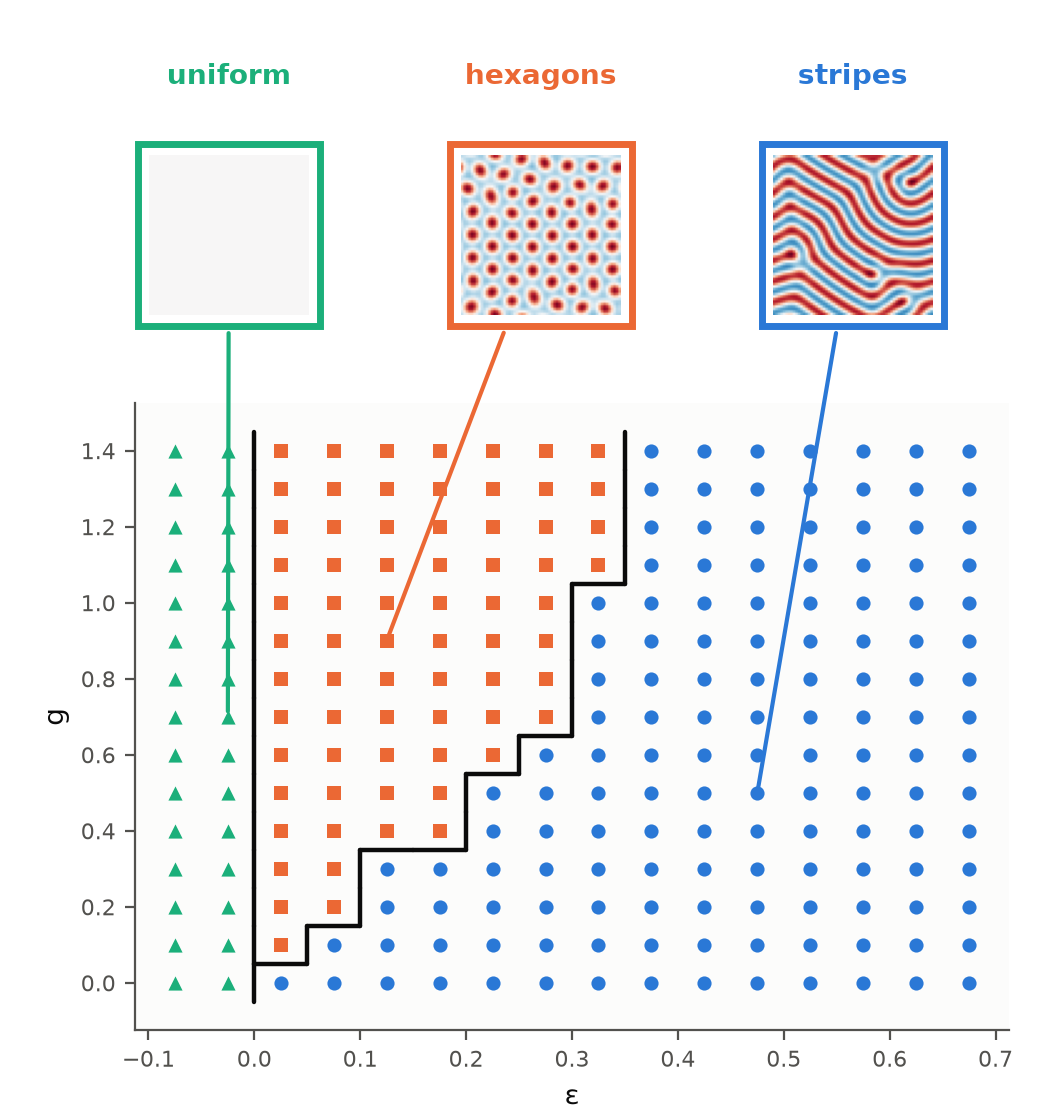
\includegraphics[height=7.0cm]{fig_sh_phases.png}};
\node[say, text width=8.3cm] at (19.6,-1.5) {
\textbf{Example: Swift-Hohenberg}, a model of pattern formation\\[2pt]
$\partial_t u=\varepsilon u-(1+\nabla^2)^2u+g\,u^2-u^3$\\[6pt]
$\bullet$ 240 parameter points $\times$ 8 runs (random starts)\\[2pt]
$\bullet$ each run: snapshots of a field $u(x,y)$\\[2pt]
$\bullet$ the method never sees the state names\\[2pt]
$\bullet$ result: 3 phases, 237 of 240 points correct\\[2pt]
$\bullet$ the walls follow the true boundaries\\[8pt]
\textbf{Idea}: a wall between two neighbouring points where the snapshots change \emph{more than they vary between runs of one point}.};

% ---------------- how: four steps
\node[anchor=north west, font=\bfseries\normalsize] at (0,-8.75) {How};
\foreach \x in {0, 7.2, 14.4, 21.6} { \draw[box] (\x,-9.3) rectangle ++(6.75,-5.6); }
\foreach \x in {6.75, 13.95, 21.15} { \draw[->, line width=1.2pt, cInk2] (\x+0.04,-12.1) -- (\x+0.41,-12.1); }

% 1 runs
\node[num] at (0.3,-9.6) {1}; \node[head] at (0.5,-9.4) {Runs on a grid};
\foreach \i in {0,...,4} \foreach \j in {0,...,3} { \fill[cInk2] (0.9+0.6*\i,-12.8+0.55*\j) circle (1.6pt); }
\draw[->] (0.7,-13.2) -- (3.75,-13.2) node[right, font=\scriptsize] {$\varepsilon$};
\draw[->] (0.5,-13.0) -- (0.5,-10.85) node[above, font=\scriptsize] {$g$};
\draw[cAcc, line width=0.8pt] (2.7,-11.7) circle (4pt);
\foreach \k in {0,1,2} { \node[tile, fill=white] (t\k) at (4.6+0.18*\k,-10.6-0.18*\k) {}; }
\begin{scope} \clip (t2.south west) rectangle (t2.north east);
  \foreach \s in {-0.3,-0.15,...,0.31} \draw[cPos!70, line width=1.1pt] ($(t2.center)+(\s,-0.3)$) -- ++(0.12,0.6);
\end{scope}
\draw[cAcc, ->] (2.85,-11.6) to[bend left=20] (4.4,-11.1);
\node[small, anchor=north] at (4.95,-11.15) {several runs\\(random starts)};
\node[say, text width=6.4cm] at (0.15,-13.5) {Snapshots of the fields of every run.};

% 2 describe
\node[num] at (7.5,-9.6) {2}; \node[head] at (7.7,-9.4) {Snapshot $\to$ vector $h$};
\node[tile, minimum size=0.75cm, fill=white] (snap) at (8.0,-11.4) {};
\begin{scope} \clip (snap.south west) rectangle (snap.north east);
  \foreach \a in {0,...,3} \foreach \b in {0,...,3} \fill[cPos!65] ($(snap.south west)+(0.1+0.19*\a,0.1+0.19*\b)$) circle (0.055);
\end{scope}
\node[blk, text width=2.6cm, font=\scriptsize] (hm) at (10.4,-10.55) {\textbf{hand-made}: spectrum, moments, domain counts, dynamics};
\node[blk, text width=2.6cm, font=\scriptsize] (le) at (10.4,-12.2) {\textbf{learned}: CNN, self-supervised (page 2)};
\draw[->] (snap.east) -- (hm.west); \draw[->] (snap.east) -- (le.west);
\foreach \k/\hh in {0/0.35,1/0.7,2/0.2,3/0.55,4/0.9,5/0.4} \fill[cP0!80] (12.55+0.12*\k,-11.8) rectangle ++(0.09,\hh);
\node[font=\scriptsize] at (12.85,-12.05) {$h$};
\draw[->] (hm.east) -- (12.5,-11.15); \draw[->] (le.east) -- (12.5,-11.55);
\node[say, text width=6.4cm] at (7.35,-13.5) {Same $h$ if the box is rotated, mirrored or shifted.};

% 3 compare and cut
\node[num] at (14.7,-9.6) {3}; \node[head] at (14.9,-9.4) {Compare neighbours, cut};
\begin{scope}[shift={(15.1,-11.6)}]
  \fill[cP0!10, draw=cP0] (0,0.35) circle (0.42); \fill[cP1!10, draw=cP1] (0,-1.05) circle (0.42);
  \foreach \p in {(-0.2,0.5),(0.1,0.6),(0.15,0.25),(-0.1,0.15),(0.2,0.45)} \fill[cP0] \p circle (1.4pt);
  \foreach \p in {(-0.15,-0.9),(0.15,-0.85),(0.1,-1.2),(-0.2,-1.15),(0.2,-1.05)} \fill[cP1] \p circle (1.4pt);
  \draw[<->, line width=0.8pt] (0,-0.1) -- node[right, font=\scriptsize] {$J$} (0,-0.6);
\end{scope}
\begin{scope}[shift={(16.75,-12.6)}]
  \foreach \i in {0,...,5} \foreach \j in {0,...,3} {
    \pgfmathtruncatemacro{\side}{(\i + 0.6*\j > 2.6) ? 1 : 0}
    \ifnum\i<5 \pgfmathtruncatemacro{\sideR}{(\i+1 + 0.6*\j > 2.6) ? 1 : 0}
      \ifnum\side=\sideR \draw[cGrid, line width=0.6pt] (0.55*\i,0.55*\j) -- ++(0.55,0); \else \draw[cInk, line width=1.8pt] (0.55*\i,0.55*\j) -- ++(0.55,0); \fi \fi
    \ifnum\j<3 \pgfmathtruncatemacro{\sideU}{(\i + 0.6*(\j+1) > 2.6) ? 1 : 0}
      \ifnum\side=\sideU \draw[cGrid, line width=0.6pt] (0.55*\i,0.55*\j) -- ++(0,0.55); \else \draw[cInk, line width=1.8pt] (0.55*\i,0.55*\j) -- ++(0,0.55); \fi \fi }
  \foreach \i in {0,...,5} \foreach \j in {0,...,3} {
    \pgfmathtruncatemacro{\side}{(\i + 0.6*\j > 2.6) ? 1 : 0}
    \ifnum\side=0 \fill[cP0] (0.55*\i,0.55*\j) circle (2.2pt); \else \fill[cP1] (0.55*\i,0.55*\j) circle (2.2pt); \fi }
  \draw[wall] (1.375,-0.275) -- (1.375,0.825) -- (0.825,0.825) -- (0.825,1.375) -- (0.275,1.375) -- (0.275,1.925);
  \node[font=\scriptsize, cAcc, anchor=west] at (0.35,2.05) {wall};
  \node[font=\scriptsize, anchor=west, align=left] at (3.0,0.8) {thick link:\\big $J$};
\end{scope}
\node[say, text width=6.4cm] at (14.55,-13.5) {$J$: distance between the clouds of $h$ of two neighbours (energy distance). Spectral cut where $J$ is large.};

% 4 test
\node[num] at (21.9,-9.6) {4}; \node[head] at (22.1,-9.4) {Test the wall};
\begin{scope}[shift={(22.35,-12.1)}]
  \draw[->] (0,0) -- (5.6,0) node[right, font=\scriptsize] {$J$};
  \foreach \xx/\hh in {0.3/0.35,0.6/0.9,0.9/1.25,1.2/0.85,1.5/0.4,1.8/0.15} \fill[cGrid] (\xx,0) rectangle ++(0.27,\hh);
  \foreach \xx/\hh in {2.9/0.2,3.2/0.55,3.5/0.8,3.8/0.6,4.1/0.3} \fill[cAcc!80] (\xx,0) rectangle ++(0.27,\hh);
  \node[font=\scriptsize, cInk2] at (1.15,1.45) {inside a phase};
  \node[font=\scriptsize, cAcc] at (3.7,1.05) {across the wall};
\end{scope}
\node[say, text width=6.4cm] at (21.75,-13.5) {Kept if jumps across $\gg$ jumps inside, measured on \emph{other runs} (below). Then cut again on each side.};

% ---------------- the key trick
\node[anchor=north west, font=\bfseries\normalsize] at (0,-15.25) {The key trick: place the wall with half of the runs, test it with the other half};
\begin{scope}[shift={(0.3,-18.95)}]
  \foreach \i in {0,...,6} \foreach \j in {0,...,3} {
    \pgfmathsetmacro{\r}{0.4+1.4*rnd}
    \ifnum\i<6 \draw[cInk2, line width=\r pt] (0.5*\i,0.5*\j) -- ++(0.5,0); \fi
    \ifnum\j<3 \pgfmathsetmacro{\q}{0.4+1.4*rnd} \draw[cInk2, line width=\q pt] (0.5*\i,0.5*\j) -- ++(0,0.5); \fi }
  \foreach \i in {0,...,6} \foreach \j in {0,...,3} \fill[cP0] (0.5*\i,0.5*\j) circle (1.8pt);
\end{scope}
\node[font=\footnotesize, anchor=north west, align=left] at (0.2,-15.85) {pure noise: no phase,\\random jumps};
\begin{scope}[shift={(5.1,-18.95)}]
  \foreach \i in {0,...,6} \foreach \j in {0,...,3} { \pgfmathtruncatemacro{\s}{\i>2 ? 1 : 0}
    \ifnum\s=0 \fill[cP0] (0.5*\i,0.5*\j) circle (1.8pt); \else \fill[cP1] (0.5*\i,0.5*\j) circle (1.8pt); \fi }
  \draw[wall] (1.25,-0.2) -- (1.25,1.7);
\end{scope}
\node[font=\footnotesize, anchor=north west, align=left, text width=4.4cm] at (5.0,-15.85) {\textbf{same runs} place and test: a fake wall in \textbf{half} of the noise tables};
\begin{scope}[shift={(10.6,-18.95)}]
  \foreach \i in {0,...,6} \foreach \j in {0,...,3} \fill[cP0] (0.5*\i,0.5*\j) circle (1.8pt);
  \draw[wall, dashed, cAcc!50] (1.25,-0.2) -- (1.25,1.7);
  \node[font=\scriptsize, cAcc] at (2.4,1.95) {rejected};
\end{scope}
\node[font=\footnotesize, anchor=north west, align=left, text width=4.4cm] at (10.5,-15.85) {half A places, \textbf{half B tests}: no wall in \textbf{140 of 140} noise or drift tables};
\node[say, text width=12.4cm] at (15.7,-15.85) {$\bullet$ Selection bias: never test a hypothesis on the data that suggested it.\\[3pt]
$\bullet$ Price: some power (a weak wall can be missed).\\[3pt]
$\bullet$ Tables with 2 or 3 true phases are still found.\\[3pt]
$\bullet$ Two thresholds only ($p<10^{-3}$, jump ratio $\ge1.5$); same result for ratios 1.2 to 2.};
\end{tikzpicture}}

\newpage
%====================================================================== page 2
\noindent\resizebox{\linewidth}{!}{%
\begin{tikzpicture}[x=1cm,y=1cm,>={Stealth}]
\node[anchor=north west, font=\bfseries\Large] at (0,0) {The learned description, other methods, and examples};

% ---------------- learned description
\draw[box] (0,-0.8) rectangle (28.3,-7.6);
\node[anchor=north west, font=\bfseries\normalsize] at (0.15,-0.9) {The learned description: a CNN trained without labels (contrastive, as SimCLR)};
% views
\node[anchor=north west, font=\bfseries\small] at (0.25,-1.55) {Views: what the network must not see};
\stripes{(1.0,-3.9)}{0.55}{0}{0.22}{70}
\node[small, anchor=north] at (1.0,-4.5) {one snapshot};
\stripes{(3.4,-2.65)}{0.42}{35}{0.22}{70}   \node[small, anchor=west] at (3.95,-2.65) {turned (any angle)};
\stripes{(3.4,-3.65)}{0.42}{0}{0.30}{70}    \node[small, anchor=west] at (3.95,-3.65) {zoomed ($\pm25\%$)};
\stripes{(3.4,-4.65)}{0.28}{0}{0.22}{70}    \node[small, anchor=west] at (3.95,-4.65) {cropped ($\frac34$ of the box)};
\stripes{(3.4,-5.65)}{0.42}{0}{0.22}{30}    \node[small, anchor=west] at (3.95,-5.65) {rescaled (own std)};
\foreach \y in {-2.65,-3.65,-4.65,-5.65} \draw[->, cInk2] (1.6,-3.9) -- (2.9,\y);
\node[say, text width=6.3cm] at (0.25,-6.2) {Two random views of the same run must give nearby $h$: orientation, wavelength, position and amplitude are not used.};
% CNN
\node[anchor=north west, font=\bfseries\small] at (7.6,-1.55) {Network};
\begin{scope}[shift={(7.9,-3.95)}]
  \foreach \k/\s/\w/\lab in {0/1.5/0.12/{64$^2$\\2},1/1.15/0.3/{32$^2$\\32},2/0.85/0.45/{16$^2$\\64},3/0.6/0.6/{8$^2$\\128},4/0.42/0.75/{4$^2$\\256}} {
    \pgfmathsetmacro{\xx}{1.05*\k}
    \fill[cP0!12, draw=cP0] (\xx,-\s/2) rectangle ++(\w,\s);
    \node[font=\tiny, align=center, anchor=north] at (\xx+\w/2,-0.85) {\lab};
  }
  \node[font=\tiny, anchor=north east, align=right] at (-0.35,-0.85) {grid:\\channels:};
  \foreach \k in {0,...,3} \draw[->, cInk2] ({1.05*\k+0.12+0.15*\k+0.05},0) -- ({1.05*(\k+1)-0.05},0);
  \node[font=\scriptsize, align=center] at (2.4,1.05) {4 convolution blocks, each halves the grid};
  \node[blk, font=\scriptsize] (mean) at (5.75,0) {mean};
  \draw[->] (4.97,0) -- (mean.west);
  \node[font=\scriptsize, align=center] (hh) at (6.65,0) {$h$\\[-2pt]{\tiny 256}};
  \draw[->] (mean.east) -- (hh.west);
  \node[blk, font=\scriptsize] (gg) at (7.55,0) {$g$};
  \draw[->] (hh.east) -- (gg.west);
  \draw[cInk2] (8.85,0) circle (0.62);
  \draw[->] (gg.east) -- (8.2,0);
  \fill[cP1] (8.65,0.3) circle (2.2pt); \fill[cP1] (8.85,0.36) circle (2.2pt);
  \fill[cP0] (9.25,-0.3) circle (2.2pt); \fill[cP2] (8.45,-0.35) circle (2.2pt);
  \node[font=\tiny, align=center, anchor=north] at (8.85,-0.7) {$z$ on a sphere};
\end{scope}
\node[say, text width=10.0cm] at (7.6,-5.65) {$\bullet$ Loss (InfoNCE): views of one run together, other runs apart.\\[2pt]
$\bullet$ After training, $g$ is dropped; $h$ replaces the hand-made vector.\\[2pt]
$\bullet$ Swift-Hohenberg: 3 phases for 3 training seeds (same as hand-made).};
% why rescale
\node[anchor=north west, font=\bfseries\small] at (18.4,-1.55) {Why rescale each view};
\begin{scope}[shift={(18.6,-5.8)}]
  \draw[->] (0,0) -- (3.9,0) node[right, font=\scriptsize] {$\varepsilon$};
  \draw[->] (0,0) -- (0,3.0);
  \fill[cP1!15] (0.3,0) rectangle (1.7,2.8); \fill[cP0!15] (1.7,0) rectangle (3.7,2.8);
  \draw[cInk, line width=1.1pt, domain=0.3:3.7, samples=40] plot (\x, {0.3+1.2*sqrt(\x-0.3)});
  \node[font=\scriptsize, anchor=west] at (0.05,2.85) {amplitude: smooth};
  \node[font=\scriptsize, cP1] at (1.0,0.25) {hex.}; \node[font=\scriptsize, cP0] at (2.7,0.25) {stripes};
\end{scope}
\begin{scope}[shift={(23.6,-5.8)}]
  \draw[->] (0,0) -- (3.9,0) node[right, font=\scriptsize] {$\varepsilon$};
  \draw[->] (0,0) -- (0,3.0);
  \fill[cP1!15] (0.3,0) rectangle (1.7,2.8); \fill[cP0!15] (1.7,0) rectangle (3.7,2.8);
  \draw[cInk, line width=1.1pt] (0.3,2.1) -- (1.7,2.1); \draw[cInk, line width=1.1pt] (1.7,0.7) -- (3.7,0.7);
  \draw[cInk, dotted] (1.7,2.1) -- (1.7,0.7);
  \node[font=\scriptsize, anchor=west] at (0.05,2.85) {shape: jumps};
  \node[font=\scriptsize, cP1] at (1.0,0.25) {hex.}; \node[font=\scriptsize, cP0] at (2.7,0.25) {stripes};
\end{scope}
\node[say, text width=9.4cm] at (18.4,-6.25) {Without rescaling, $h$ followed the amplitude: 2 phases of 3.\\With it, $h$ follows the shape: 3 of 3.};

% ---------------- other methods on the same h
\draw[box] (0,-7.9) rectangle (28.3,-11.75);
\node[anchor=north west, font=\bfseries\normalsize] at (0.15,-8.0) {Other ways to group the same $h$ (all label-free), on Swift-Hohenberg};
% walls
\begin{scope}[shift={(0.6,-11.05)}]
  \foreach \i in {0,...,5} \foreach \j in {0,...,3} { \pgfmathtruncatemacro{\s}{(\i + 0.6*\j > 2.6) ? 1 : 0}
    \ifnum\s=0 \fill[cP0] (0.4*\i,0.4*\j) circle (1.8pt); \else \fill[cP1] (0.4*\i,0.4*\j) circle (1.8pt); \fi }
  \draw[wall] (1.0,-0.2) -- (1.0,0.6) -- (0.6,0.6) -- (0.6,1.0) -- (0.2,1.0) -- (0.2,1.4);
\end{scope}
\node[say, text width=5.6cm] at (3.3,-8.7) {\textbf{Walls} (this method): cuts along the parameter grid, each tested.\\[2pt]ARI 0.93 hand-made, 0.96 learned; 3 connected phases.};
% tree
\begin{scope}[shift={(10.6,-8.85)}]
  \node[blk, font=\tiny] (r1) at (0,0) {variance of $u\approx0$?};
  \node[font=\tiny, cP2, anchor=north] (a1) at (-1.15,-0.75) {uniform};
  \node[blk, font=\tiny] (r2) at (1.0,-0.95) {many small low domains?};
  \node[font=\tiny, cP1, anchor=north] at (0.1,-1.75) {hexagons};
  \node[font=\tiny, cP0, anchor=north] at (2.0,-1.75) {stripes};
  \draw[->] (r1) -- node[left, font=\tiny] {yes} (a1); \draw[->] (r1) -- node[right, font=\tiny] {no} (r2);
  \draw[->] (r2) -- (0.1,-1.72); \draw[->] (r2) -- (2.0,-1.72);
\end{scope}
\node[say, text width=5.0cm] at (13.45,-8.7) {\textbf{Threshold tree}: phases as rules on single observables, each split tested.\\[2pt]ARI 0.94; the rules read as physics.};
% blind clustering
\begin{scope}[shift={(19.9,-10.1)}]
  \foreach \p in {(0,0.2),(0.2,0.4),(0.3,0.05),(0.1,-0.1),(-0.15,0.3)} \fill[cP0] \p circle (1.6pt);
  \foreach \p in {(0.65,0.35),(0.85,0.5),(0.95,0.2),(0.7,0.05),(1.05,0.4)} \fill[cP1] \p circle (1.6pt);
  \foreach \p in {(1.6,-0.4),(1.75,-0.2),(1.9,-0.45),(1.7,-0.6)} \fill[cP2] \p circle (1.6pt);
  \foreach \p in {(0.45,-0.5),(1.3,0.7),(1.3,-0.1)} \fill[cGrid] \p circle (1.6pt);
  \node[font=\tiny, anchor=north] at (0.9,-0.75) {clouds of $h$ (grey: noise)};
\end{scope}
\node[say, text width=5.6cm] at (22.4,-8.7) {\textbf{Blind clustering} (Gaussian mixture, k-means, HDBSCAN): ignores the grid.\\[2pt]ARI 0.38-0.78: phases cut in bands or 12-49\% of runs left as noise. Needs separated clouds; the walls only need a jump between neighbours.};

% ---------------- works: Gray-Scott
\draw[draw=cOK, line width=1.2pt, rounded corners=4pt, fill=cOK!3] (0,-12.05) rectangle (13.95,-19.6);
\node[anchor=north west, font=\bfseries\normalsize, cOK] at (0.15,-12.15) {Works: Gray-Scott reaction-diffusion};
\node[anchor=north west, inner sep=0] at (0.2,-12.7) {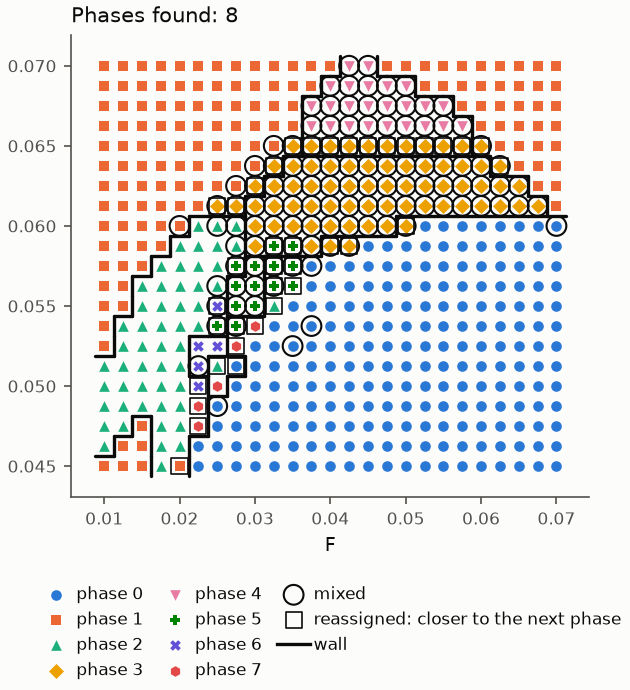
\includegraphics[height=4.4cm]{gs_map.png}};
\node[say, text width=9.2cm] at (4.5,-12.8) {$\bullet$ 525 points $\times$ 4 runs, hand-made $h$\\[2pt]
$\bullet$ 8 phases: two uniform states, spots, stripes, moving patterns, isolated spots\\[2pt]
$\bullet$ ARI 0.89 with the known diagram\\[2pt]
$\bullet$ rings: mixed points, where runs disagree\\[2pt]
$\bullet$ snapshots: one per phase found (frame = phase colour)};
\node[anchor=north west, inner sep=0] at (0.2,-17.35) {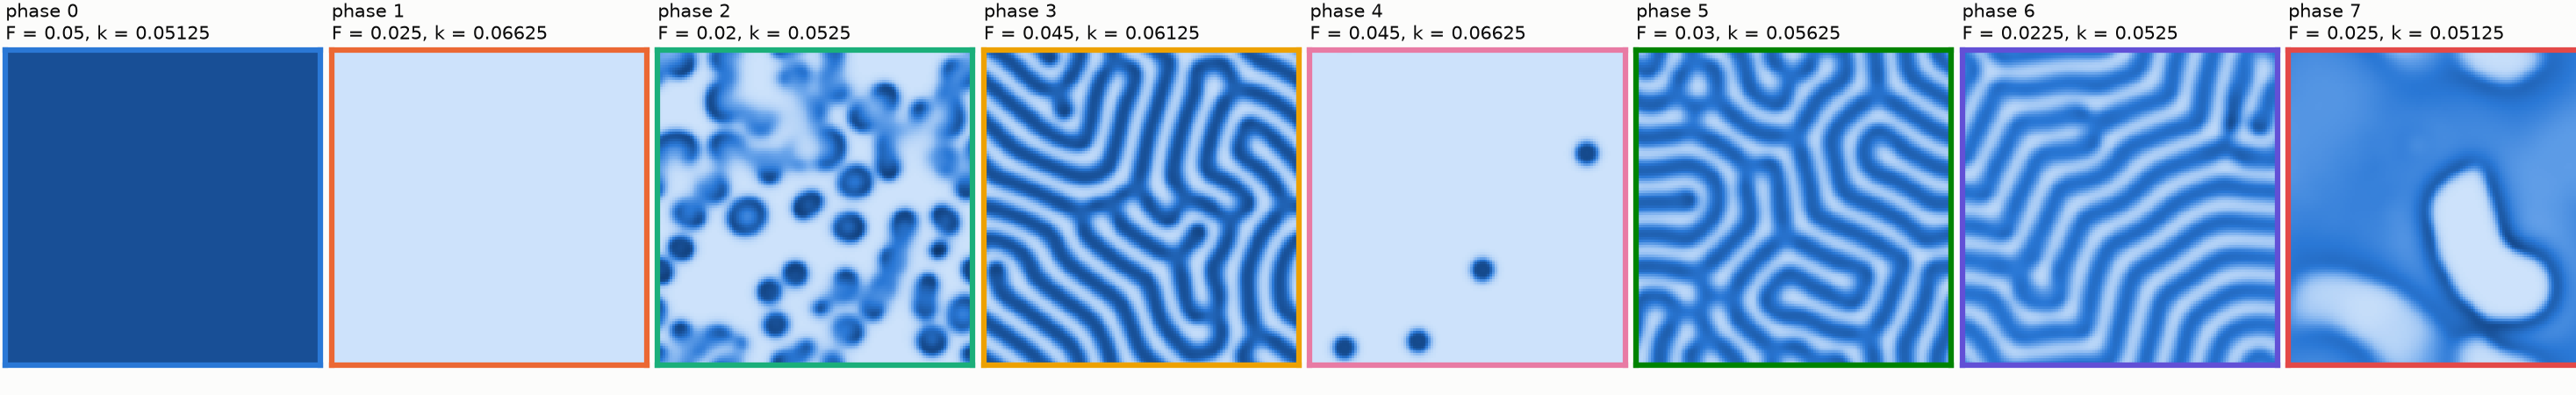
\includegraphics[width=13.5cm]{gs_phases.png}};

% ---------------- fails: Barkley
\draw[draw=cBad, line width=1.2pt, rounded corners=4pt, fill=cBad!3] (14.35,-12.05) rectangle (28.3,-19.6);
\node[anchor=north west, font=\bfseries\normalsize, cBad] at (14.5,-12.15) {Partly fails: Barkley excitable medium (waves)};
\node[anchor=north west, inner sep=0] at (14.5,-12.7) {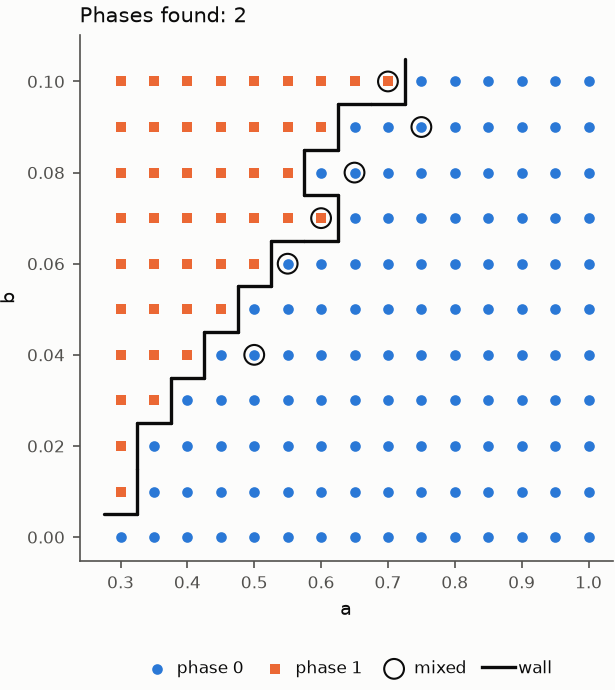
\includegraphics[height=4.2cm]{barkley_map.png}};
\node[anchor=north west, inner sep=0] at (18.3,-12.7) {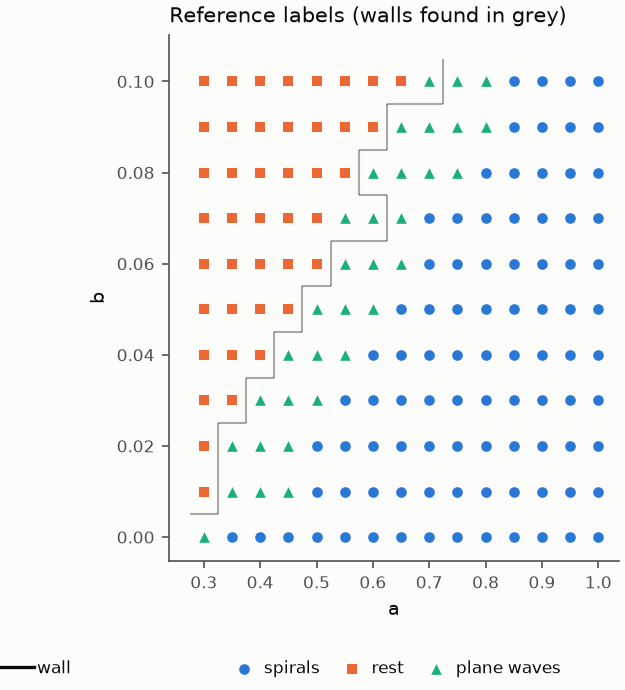
\includegraphics[height=4.2cm]{barkley_ref.png}};
\node[font=\scriptsize\bfseries, anchor=north] at (16.4,-16.9) {walls: 2 phases};
\node[font=\scriptsize\bfseries, anchor=north] at (20.2,-16.9) {known: 3 states};
\node[anchor=north west, inner sep=0] at (22.35,-12.75) {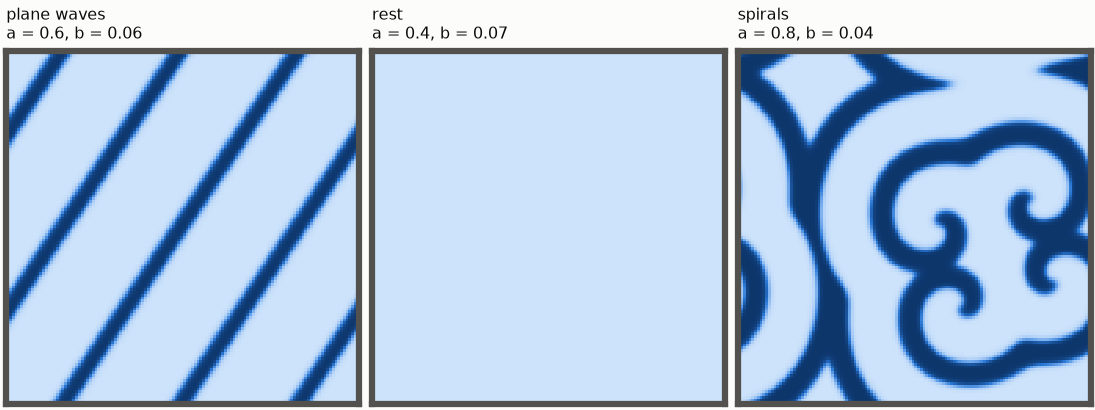
\includegraphics[width=5.8cm]{barkley_states.png}};
\node[anchor=north west, inner sep=0] at (23.0,-15.0) {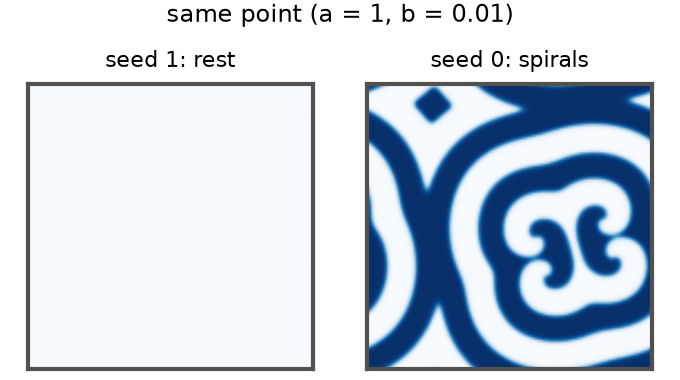
\includegraphics[width=4.4cm]{fig_barkley_mixed.png}};
\node[say, text width=13.5cm] at (14.5,-17.6) {$\bullet$ Found: rest against activity. Missed: plane waves against spirals.\\[2pt]
$\bullet$ Why: at 52 of 165 points the runs end in different states (right). Spread within a point $\approx$ jump between points: no wall passes the test.\\[2pt]
$\bullet$ Assumption broken: \emph{one state per point}. Next: describe a point as a mixture of states.};

\node[anchor=north west, font=\tiny, cInk2, text width=28cm] at (0,-19.75) {PhaseWall, Ludovic Dumoulin, November 2026. Python (NumPy, SciPy, PyTorch); 210 tests; details in docs/documentation.pdf. ARI: adjusted Rand index against the known states (1: identical, 0: chance). The code, tests and documentation were written by Claude (Anthropic), an AI assistant; the author designed the method, chose the physics, the examples and the checks, directed the work and reviewed the results.};
\end{tikzpicture}}
\end{document}
